% When Perplexity Lies — ACL/ARR submission source.
%
% Compiles out of the box with a plain single-column fallback. `acl.sty` and `acl_natbib.bst`
% (from the ROOT of https://github.com/acl-org/acl-style-files — not a latex/ subdirectory)
% are committed alongside this file, so the \IfFileExists switch below selects the real ACL
% two-column layout. Delete them to proof-read in the fallback.
%
% ANONYMITY: this source is anonymous, as ARR requires. See the marked blocks below for
% where to add author information and the artifact link when preparing a camera-ready.

\documentclass[11pt]{article}

\IfFileExists{acl.sty}{%
  \usepackage[review]{acl}%
}{%
  % ---- fallback: compiles anywhere with standard packages -------------------
  % Layout differs from ACL's, but every macro used below resolves, so the source
  % can be proof-read and checked for undefined references without the style files.
  \usepackage[letterpaper,margin=1in]{geometry}
  \usepackage{times}
  \usepackage{natbib}
  \bibliographystyle{plainnat}
  \setlength{\bibsep}{2pt}
  % acl.sty loads hyperref itself (plain), so loading it with options here would be an
  % option clash under the real style. Fallback-only.
  \usepackage[hidelinks]{hyperref}
  \newcommand{\aclfallback}{}
}

\usepackage[T1]{fontenc}
\usepackage[utf8]{inputenc}
% expansion=false: the fallback's Type1 `times` is not scalable, and font expansion errors
% out on it. Protrusion (the main visual benefit) still applies, and this is safe under the
% official ACL style too.
\usepackage[expansion=false]{microtype}
\usepackage{graphicx}
\usepackage{booktabs}
\usepackage{amsmath}
\usepackage{amssymb}
\usepackage{xcolor}
\usepackage{url}

\graphicspath{{figures/}}

% Captions carry long unbreakable tokens (\texttt{acc\_norm}, model names like Llama-3.2-3B)
% that cannot hyphenate in a narrow ACL column. Let TeX stretch interword space as a last
% resort rather than push text into the margin.
\setlength{\emergencystretch}{1.5em}

\newcommand{\ppl}{\mbox{PPL}}
\newcommand{\best}[1]{\textbf{#1}}

\title{When Perplexity Lies: A Controlled Perplexity Collapse\\
       with No Downstream Degradation in Weight-Quantized LLMs}

% ---- ANONYMOUS (ARR). For camera-ready, replace with the real author block. ----
\author{Anonymous ARR submission}

\begin{document}
\maketitle

\begin{abstract}
Post-training quantization of large language models is evaluated overwhelmingly by WikiText
perplexity, and perplexity regressions are routinely read as utility loss. We show this
inference can fail badly. Using outlier-channel protection---keeping a small fraction of input
channels in FP16 on a low-bit base---we construct a controlled generator of extreme perplexity
damage: on an error-compensated GPTQ-4 base, a selector that ranks channels by the
Hessian-weighted residual objective raises Llama-3.2-3B WikiText-2 perplexity from 8.17 to
51.68 at matched weight-only storage. Disk reload verifies the evaluated checkpoint is that
model (51.76). Yet on six zero-shot tasks it loses nothing: macro accuracy 67.61\% versus
67.10\% for its own base, a paired-bootstrap difference of $+0.51$ points whose interval
excludes zero, and LAMBADA perplexity 4.17. The pattern replicates on Llama-3.2-1B (10.56 to
63.83 reload-verified, $+0.32$ points). A per-token decomposition rules out the obvious
explanation: the damage is broad, not a tail artifact---74.6\% of tokens degrade, the median
token worsens, and excluding the worst 5\% still leaves a $4\times$ gap. We further show the
damage requires the selector's off-diagonal Hessian coupling, and refute the natural mechanism:
scored by its exact objective, the harmful selector is \emph{anti}-correlated with the base's
error compensation while the safest selector tracks it almost perfectly.
\end{abstract}

\section{Introduction}
\label{sec:intro}

Weight-only post-training quantization (PTQ) is the default way to shrink large language
models, and the field's default report is a WikiText perplexity table. Methods are accepted or
rejected on perplexity deltas that are often far smaller than one point, and deployment gates
are frequently written in the same terms. Implicit in this practice is an assumption: that
perplexity movement tracks the model's usefulness.

We show that assumption can fail by a wide margin, using a construction entirely within
standard PTQ practice. \emph{Outlier-channel protection}---keeping a small fraction of input
channels in FP16 on top of a low-bit base---is a common recipe
\citep{dettmers2022llmint8,lee2024owq,dettmers2023spqr}. Its selection signal is usually
presented as a design detail. We find that one standard choice of signal, applied to an
error-compensated base, produces a catastrophic perplexity collapse: on Llama-3.2-3B with a
GPTQ-4 base \citep{frantar2023gptq}, protecting 2\% of input channels chosen by the
Hessian-weighted residual objective moves WikiText-2 perplexity from \best{8.17 to 51.68}, at
matched theoretical weight-only storage, while random selection of the same number of channels
leaves it at 8.18.

A $6.3\times$ perplexity increase would normally end the discussion. We instead treat it as an
instrument. We export that exact configuration to a dense checkpoint, verify by in-memory
materialization and by disk reload that the checkpoint \emph{is} the perplexity-51.76 model,
and then evaluate it on six standard zero-shot tasks. It shows no degradation at all: macro
accuracy \best{67.61\%} against \best{67.10\%} for its own unprotected base and \best{68.43\%}
for FP16, a paired bootstrap difference of \best{$+0.51$ points $[+0.13, +0.86]$}---
statistically \emph{favourable}---with LAMBADA perplexity \best{4.17}, comparable to the base's
4.28.

\paragraph{Contributions.}
\begin{enumerate}\itemsep2pt
\item A reload-verified demonstration that a ${\sim}6\times$ WikiText-2 perplexity collapse can
carry \textbf{zero downstream cost} on six tasks, on \textbf{two models}, including a
token-level task on a second corpus (\S\ref{sec:decouple}).
\item A \textbf{per-token decomposition falsifying the tail explanation}: the degradation is
broad (74.6\% of tokens worse, median $\Delta$NLL $+0.287$), so the decoupling is not an
artifact of a few catastrophic tokens (\S\ref{sec:pertoken}).
\item A characterization of \emph{what generates} the perplexity damage: it requires the
selector's \textbf{off-diagonal Hessian coupling}. Selectors using no Hessian, only its
diagonal, only residual magnitude, or random selection are all benign at every budget we tested
(\S\ref{sec:generates}).
\item A \textbf{falsified mechanism}, reported as such: the natural explanation---that
protection destroys the base's error compensation---predicts that harmful selectors target
compensation-bearing columns. Direct measurement shows the opposite ordering
(\S\ref{sec:falsified}).
\item A quantification of how much the effect depends on the \textbf{selector's own Hessian
estimate} (\S\ref{sec:selectorH}), and a \textbf{model-scope boundary}: two of four checkpoints
exhibit the collapse, and on Qwen2.5-3B no selector is harmful at all (\S\ref{sec:scope}).
\item Supporting audits under matched storage with random controls, including a matched-bit
downstream signal-versus-random test (\S\ref{sec:audits}).
\end{enumerate}

\paragraph{Scope of the claim.} We do not claim perplexity is uninformative, nor that this
configuration is one practitioners would deliberately choose. We claim that a perplexity gap of
this magnitude, produced by an ordinary PTQ manipulation, is not sufficient evidence of utility
loss---and that quantization studies and regression gates relying on perplexity alone can
therefore be badly miscalibrated.

\paragraph{What is not new.} Activation-outlier protection
\citep{dettmers2022llmint8}, Hessian- and error-based column selection
\citep{lee2024owq,dettmers2023spqr}, and integrating protected-column selection into the
compensation pass \citep{lee2024owq} are all prior work. Our contribution is the controlled
decoupling demonstration, the structural condition on the selector, and the negative mechanism
result.

\section{Related work}
\label{sec:related}

\paragraph{Outlier-aware mixed precision.} \citet{dettmers2022llmint8} decompose the matmul so
outlier feature dimensions stay in FP16. OWQ \citep{lee2024owq} scores input columns by
Hessian-weighted quantization error, keeps the top ones in FP16, and---crucially for our
analysis---orders them last inside the OPTQ pass, so compensation proceeds knowing which
columns remain exact. SpQR \citep{dettmers2023spqr} isolates outlier weights in a sparse
high-precision format. Atom \citep{zhao2024atom} and SqueezeLLM \citep{kim2023squeezellm} use
related group/column/row schemes; AWQ \citep{lin2024awq} scales channels by activation
statistics. Our selectors are drawn from this family; we vary the signal and the base rather
than proposing a new protector.

\paragraph{Error compensation.} GPTQ \citep{frantar2023gptq}, building on OBQ
\citep{frantar2022obc}, quantizes column by column and propagates each column's rounding error
into the not-yet-quantized columns, minimizing $\lVert \Delta W X \rVert^2$. The residual it
leaves is therefore structured, which is what makes the base$\times$selector interaction we
study non-trivial. HQQ \citep{badri2023hqq} is calibration-free but is \emph{not} plain
round-to-nearest: it optimizes quantization parameters with a half-quadratic splitting
procedure under a robust reconstruction loss.

\paragraph{Evaluating quantized models.} Broad benchmark studies
\citep{jin2024comprehensive} report downstream task results for quantized LLMs, and several
works note that perplexity and task metrics can move differently. Our contribution is sharper
and adversarial: rather than observing correlation strength across methods, we \emph{construct}
a checkpoint with an extreme perplexity gap and verify that the downstream cost is nil, which
bounds how much a perplexity delta can be trusted.

\section{Setup}
\label{sec:setup}

\paragraph{Protection form.} For a linear layer with weight $W \in \mathbb{R}^{o \times i}$ and
protected input-channel set $S$, the protected forward pass is
$y = Q(W)x + x[S]\cdot(W - Q(W))[:,S]^{\top}$. Materializing gives
$W_{\text{dense}} = Q(W) + \mathrm{scatter}(W - Q(W), S)$, algebraically identical to the
forward pass, so a faithful export must reproduce the runtime perplexity. We use this identity
as an integrity check (\S\ref{sec:identity}). Storage is additive: the low-bit base is retained
and FP16 correction columns are stored on top, rather than replacing base columns.

\paragraph{Bases.} (i)~\textbf{HQQ-4} \citep{badri2023hqq}, calibration-free, no error
compensation. (ii)~\textbf{GPTQ-4} \citep{frantar2023gptq}, error-compensated, produced at W4
group size 128 with a fixed WikiText-2 calibration set ($128 \times 2048$ tokens), imported as
fake-quantized weights and re-evaluated in our own evaluator.

\paragraph{Selectors.} With residual $\Delta W = W - Q(W)$ and input Hessian $H = X^{\top}X$,
Table~\ref{tab:selectors} lists the signals. \texttt{greedy\_indep} is a \emph{one-shot
full-Hessian} selector, not an activation-magnitude score. The last two maximize the exact
reduction in $\lVert \Delta W X\rVert^2 = \mathrm{tr}(\Delta W H \Delta W^{\top})$ obtainable
by restoring columns.

\begin{table}[t]
\centering\small
\begin{tabular}{lccc}
\toprule
selector & $\Delta W$ & $H$ diag & $H$ off-diag \\
\midrule
\texttt{random} (3 seeds)      & --- & --- & --- \\
\texttt{act\_max}, \texttt{act\_scale} & --- & --- & --- \\
\texttt{residual\_max/rms}     & \checkmark & --- & --- \\
\texttt{hessian\_diag}         & --- & \checkmark & --- \\
\texttt{greedy\_indep}         & \checkmark & \checkmark & \checkmark \\
\texttt{greedy} (iterative)    & \checkmark & \checkmark & \checkmark \\
\bottomrule
\end{tabular}
\caption{Selection signals and which parts of the objective each uses.}
\label{tab:selectors}
\end{table}

\paragraph{Storage.} We report \textbf{matched theoretical weight-only storage}: bits per
quantized-linear parameter, counting low-bit values, group scales/zeros at the base's true
group size (128 for the imported GPTQ base), FP16 correction columns and channel indices.
Embeddings, \texttt{lm\_head} and norms are FP16 in every method and excluded from the axis;
all runs exclude \texttt{lm\_head} from quantization so the quantized scope matches the
baseline exactly. No kernels, packing or latency are modelled.

\paragraph{Evaluation.} WikiText-2 \citep{merity2017pointer} perplexity, sequence length 2048,
canonical non-overlapping chunking, one evaluator for every perplexity in this paper; exported
checkpoints are evaluated after reload. Downstream: lm-evaluation-harness
\citep{eval-harness} on six zero-shot tasks---HellaSwag \citep{zellers2019hellaswag}, ARC-easy
and ARC-challenge \citep{clark2018arc}, PIQA \citep{bisk2020piqa}, WinoGrande
\citep{sakaguchi2021winogrande} and LAMBADA \citep{paperno2016lambada}---on full test sets, with
paired-bootstrap 95\% confidence intervals on per-example correctness. The imported GPTQ base
measures 10.557 on Llama-3.2-1B in our evaluator versus 10.363 as reported by the producing
toolkit, so we use the \textbf{reloaded $k=0$ checkpoint} as the operational base for every
contrast, keeping all comparisons inside one evaluator.

\paragraph{Calibration provenance.} The base quantizer's Hessian came from
$128 \times 2048 \approx 262$k WikiText-2 tokens. Our selectors' Hessian, by default, came from
a 51-prompt instruction set of ${\approx}500$ tokens---rank-deficient for layers with
3072--8192 input channels, and a different distribution. We treat this as an experimental
variable rather than a fixed detail, and measure its effect in \S\ref{sec:selectorH}.

\section{A perplexity collapse with no downstream cost}
\label{sec:decouple}

\subsection{The two measurements}
\label{sec:measurements}

On Llama-3.2-3B with the GPTQ-4 base (8.172 in our evaluator, 4.25 bits), protecting 2\% of
input channels with \texttt{greedy} gives 51.68 perplexity at 4.57 bits. Entries in
Table~\ref{tab:operating} share identical storage at a given budget.

\begin{table}[t]
\centering\footnotesize\setlength{\tabcolsep}{3.5pt}
\resizebox{\columnwidth}{!}{%
\begin{tabular}{lrrr}
\toprule
point & WT2 \ppl & acc & LAMB. \\
\midrule
FP16                    & 7.817  & 68.43\% & --- \\
GPTQ-4 (base)           & 8.172  & 67.10\% & 4.28 \\
\best{greedy@GPTQ, 2\%} & \best{51.68} & \best{67.61\%} & \best{4.17} \\
resmax@GPTQ, 2\%        & 8.100  & 67.47\% & --- \\
HQQ-4 (base)            & 8.328  & 66.86\% & --- \\
best greedy@HQQ, 20\%   & 7.994  & 68.14\% & --- \\
random@HQQ, 20\%        & 8.247  & 67.21\% & --- \\
\bottomrule
\end{tabular}}
\caption{Llama-3.2-3B operating points. \emph{acc} is macro accuracy over six tasks
(\texttt{acc\_norm} where the task provides it, \texttt{acc} otherwise); \emph{LAMB.} is LAMBADA
perplexity. Both come from the same artifact the confidence intervals are computed from.}
\label{tab:operating}
\end{table}

\begin{table}[t]
\centering\footnotesize\setlength{\tabcolsep}{3.5pt}
\resizebox{\columnwidth}{!}{%
\begin{tabular}{lrl}
\toprule
contrast & $\Delta$ (pts) & 95\% CI \\
\midrule
\best{greedy@GPTQ $-$ GPTQ-4} & \best{$+0.51$} & \best{$[+0.13, +0.86]$} \\
resmax@GPTQ $-$ GPTQ-4        & $+0.37$ & $[-0.06, +0.77]$ \\
best@HQQ $-$ HQQ-4            & $+1.28$ & $[+0.84, +1.68]$ \\
best@HQQ $-$ random@HQQ       & $+0.92$ & $[+0.50, +1.34]$ \\
\bottomrule
\end{tabular}}
\caption{Paired-bootstrap macro-$\Delta$ accuracy, Llama-3.2-3B.}
\label{tab:contrasts}
\end{table}

The model whose perplexity rose $6.3\times$ is \emph{not} worse downstream; its confidence
interval against its own base excludes zero on the favourable side. Its LAMBADA perplexity---a
token-level metric on a different corpus---is 4.17, slightly better than the base's 4.28.
Figure~\ref{fig:decoupling} shows the whole picture.

\begin{figure}[t]
\centering
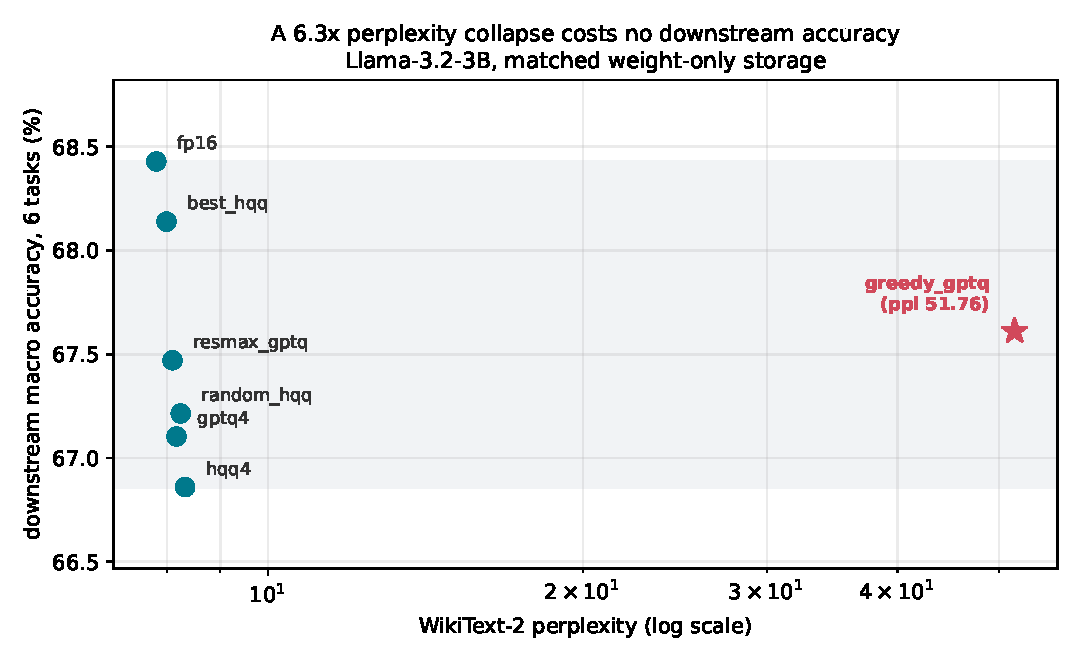
\includegraphics[width=\columnwidth]{fig0_decoupling.pdf}
\caption{Every operating point of Llama-3.2-3B: WikiText-2 perplexity (log) against downstream
macro accuracy. The catastrophic point sits $6.3\times$ to the right yet at the same height,
above both the GPTQ-4 and HQQ-4 bases.}
\label{fig:decoupling}
\end{figure}

\subsection{The checkpoint is the same model}
\label{sec:identity}

Because this is the crux, we establish checkpoint identity explicitly. The protection form
guarantees $\ppl_{\text{runtime}} = \ppl_{\text{materialized}}$ algebraically
(\S\ref{sec:setup}), and we confirm it empirically at each stage of the chain that produced the
downstream number: in-sweep runtime 51.68; in-memory materialization 51.76; the exported
checkpoint reloaded from disk \best{51.76} (\textsc{pass}, tolerance 0.5); the same directory
scored by lm-evaluation-harness, macro \best{67.61\%}. The reload was run on the exact directory
the harness loaded, after the downstream evaluation.

\paragraph{It replicates on a second model.} Llama-3.2-1B reproduces the pattern under the same
verification discipline (Table~\ref{tab:replication}): the exported checkpoint reloads at
\best{63.83} against a sweep value of 63.95 (\textsc{pass}, $\Delta = 0.124$), a $6.0\times$
increase over its 10.557 base, and scores macro \best{58.67\%} against the base's \best{58.35\%}.
The interval includes zero, so on 1B we claim no degradation rather than an improvement; on 3B
the interval excludes zero on the favourable side.

\begin{table}[t]
\centering\small\setlength{\tabcolsep}{2.5pt}
\begin{tabular}{lrrl}
\toprule
model & base & greedy (reload) & macro $\Delta$ \\
\midrule
3B & 8.172  & 51.76 \textsc{(pass)} & $+0.51\,[+0.13,+0.86]$ \\
1B & 10.557 & 63.83 \textsc{(pass)} & $+0.32\,[-0.07,+0.73]$ \\
\bottomrule
\end{tabular}
\caption{Both susceptible models: a ${\sim}6\times$ perplexity collapse with no measurable
downstream cost.}
\label{tab:replication}
\end{table}

\subsection{The damage is broad, not a tail artifact}
\label{sec:pertoken}

The obvious explanation is that perplexity, being $\exp$ of a \emph{mean} negative
log-likelihood, is dominated by its worst tokens: if a small minority of tokens became
catastrophically improbable, perplexity would explode while the bulk of the model's behaviour
stayed intact. We pre-registered this hypothesis and tested it directly, scoring both
checkpoints on the identical token stream (141 windows, 288{,}627 supervised targets) and
decomposing the per-token negative log-likelihood.

\textbf{The hypothesis is false.} The degradation is broad: \best{74.6\%} of tokens have higher
NLL, 25.4\% lower, and the median $\Delta$NLL is \best{$+0.287$}. The worst 1\% of tokens carry
only 6.9\% of the total increase, and the worst 10\% only 46.3\%.
Table~\ref{tab:trimmed} gives the perplexity after excluding the worst-$k$\% of tokens for both
models.

\begin{table}[t]
\centering\small
\begin{tabular}{lrr}
\toprule
excluded & base & greedy@GPTQ \\
\midrule
0\% & 8.17 & 51.76 \\
1\% & 8.30 & 46.85 \\
5\% & 8.59 & \best{34.56} \\
\bottomrule
\end{tabular}
\caption{Trimmed perplexity, Llama-3.2-3B. Removing the worst 5\% of tokens---fifty times more
than a tail explanation would require---still leaves a $4\times$ gap.}
\label{tab:trimmed}
\end{table}

The \emph{median} token is meaningfully worse and three quarters of all tokens degrade. This is
not a small set of outliers dragging up a mean; the model is genuinely and broadly worse at
next-token prediction on WikiText-2. That makes the result more surprising, not less, and it
removes the most comfortable way to dismiss it. A model can be substantially and pervasively
worse at modelling a corpus while answering six downstream benchmarks exactly as well as
before. We do not have a positive account of why, and we do not offer one.

\section{What generates the perplexity damage}
\label{sec:generates}

\subsection{The damage requires off-diagonal Hessian coupling}
\label{sec:offdiag}

Table~\ref{tab:panel} gives all selectors at matched storage on the GPTQ-4 base at 2\%
protection. \texttt{hessian\_diag}---which uses the Hessian, but only its diagonal---is benign at
every budget we tested (3B: 8.153/8.163/8.156/8.147 at 2/5/10/20\%; 1B:
10.441/10.462/10.475/10.450). Only the two selectors using the \textbf{off-diagonal},
cross-column terms cause damage. This rules out both ``reads the quantization residual'' and
``uses the Hessian'' as the operative property and isolates the interaction structure
(Figure~\ref{fig:coupling}).

\begin{table}[t]
\centering\small
\begin{tabular}{llrr}
\toprule
selector & Hessian use & 3B & 1B \\
\midrule
\texttt{random}        & none & 8.181 & 10.41 \\
\texttt{act\_max}      & none & 8.181 & 10.71 \\
\texttt{act\_scale}    & none & 8.586 & 10.93 \\
\texttt{residual\_max} & none & 8.100 & 10.42 \\
\texttt{residual\_rms} & none & 8.146 & 10.43 \\
\texttt{hessian\_diag} & diag only & \best{8.153} & \best{10.441} \\
\texttt{greedy\_indep} & full, one-shot & 41.50 & 11.28 \\
\texttt{greedy}        & full, iterative & \best{51.68} & \best{63.95} \\
\bottomrule
\end{tabular}
\caption{All selectors at 2\%, GPTQ-4 base (3B base 8.172; 1B base 10.557).}
\label{tab:panel}
\end{table}

\begin{figure}[t]
\centering
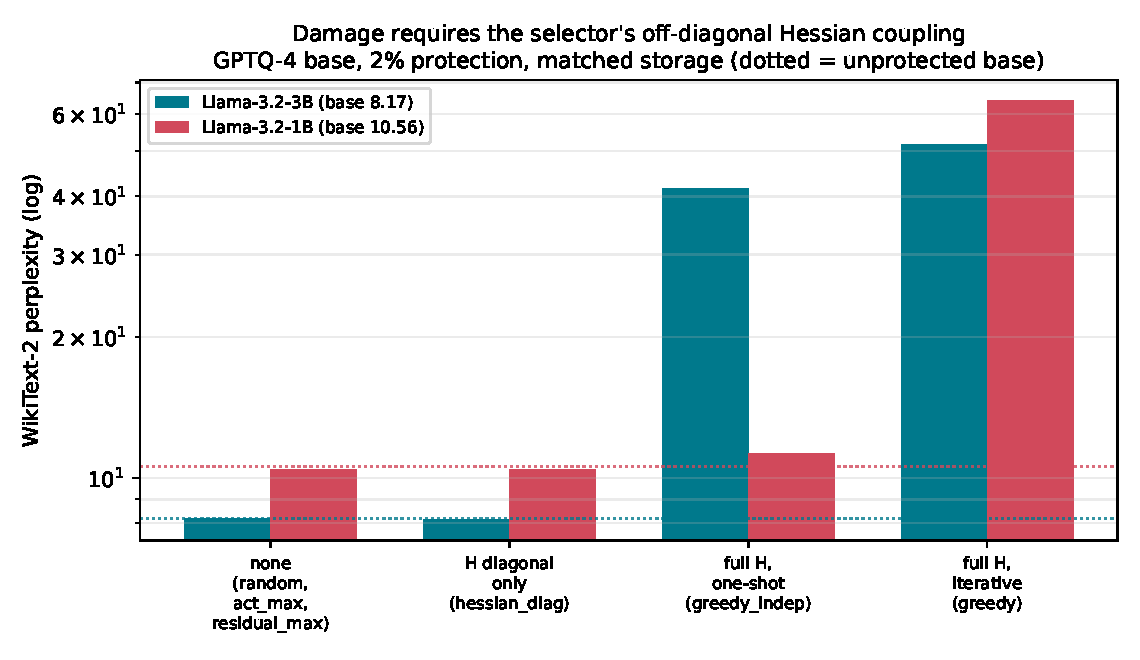
\includegraphics[width=\columnwidth]{fig5_coupling.pdf}
\caption{Perplexity by how much of the Hessian objective the selector uses. Dotted lines are the
unprotected bases.}
\label{fig:coupling}
\end{figure}

We avoid absolutes: the benign selectors are not exactly neutral. \texttt{act\_scale} reaches
8.586 at 2\% on 3B and \texttt{random} reaches 9.048 at the 10\% budget---moderate movements,
one to two orders of magnitude smaller than the collapse. Throughout we call a change
\emph{indistinguishable} within $\pm 0.1$ \ppl{} of the base, \emph{moderate} up to
${\sim}1$ \ppl, and \emph{catastrophic} above $5\times$ the base.

\subsection{Severity within the coupled selectors}

Among the two coupled selectors, iterative re-scoring is at least as harmful as one-shot
evaluation, but the separation is model-dependent and not monotone in budget. On 1B the ordering
is clean at 2\% (63.95 vs 11.28); on 3B both collapse (51.68 vs 41.50) and \texttt{greedy} is
worse at 2\% and 5\% but \emph{less} harmful at 10\% and 20\% (38.39, 40.65 vs 44.83, 43.04). We
therefore report that coupling is necessary for harm, and that harm saturates rather than
scaling smoothly once present.

\subsection{The selector's own Hessian estimate matters}
\label{sec:selectorH}

Our default selector Hessian used ${\approx}500$ tokens of out-of-distribution prompts, against
262k in-distribution tokens for the base. Re-running \texttt{greedy} with the selector Hessian
estimated from the same $128 \times 2048$ WikiText-2 tokens as the base gives 3B
$51.68 \rightarrow \best{58.24}$ and 1B $63.95 \rightarrow \best{11.39}$. On 3B the collapse
persists and is slightly worse, so it is \textbf{not} an artifact of an under-estimated Hessian.
On 1B most of it disappears (11.39 against a 10.557 base---moderate, not catastrophic), so on
that model the estimate quality was doing much of the work. Any study using Hessian-based
selection should report the selector's calibration size and distribution; we did not initially,
and it materially changes one of our two models.

\subsection{On which models the collapse occurs at all}
\label{sec:scope}

The collapse is not universal. Running the identical configuration across four checkpoints:
Llama-3.2-1B ($10.557 \rightarrow 63.95$) and Llama-3.2-3B ($8.172 \rightarrow 51.68$) collapse;
Qwen2.5-3B does not ($8.290 \rightarrow 8.335$, i.e.\ $+0.045$); Llama-2-7B does not
($5.571$ against an FP16 reference of $5.469$; its unprotected base was not measured in that
run, so we treat it as weaker evidence).

On Qwen2.5-3B the \emph{entire} selector panel is benign at 2\%---\texttt{greedy} 8.335,
\texttt{greedy\_indep} 8.357, \texttt{residual\_rms} 8.339, \texttt{residual\_max} 8.351,
\texttt{act\_max} 8.366, \texttt{act\_scale} 8.372, \texttt{random} 8.300, against a base of
8.290. The spread across every selector is under 0.09 perplexity, so on this model the choice of
selection signal is immaterial.

The collapse therefore requires the structural condition of \S\ref{sec:offdiag} \emph{and} a
susceptible model. Two of four checkpoints are, both from the same family. We have no predictor
for susceptibility, and finding one is the clearest route to turning this boundary into a
diagnostic. Note that these models cannot supply further decoupling replication: a model healthy
in perplexity has nothing to decouple, so evaluating it downstream would only confirm that a
healthy model scores healthily.

\section{A falsified mechanism}
\label{sec:falsified}

The natural explanation for \S\ref{sec:generates} is that the coupled selectors identify columns
carrying GPTQ's deposited error correction, and that restoring those columns to FP16 discards
compensation the remaining columns were tuned around. This predicts that harmful selectors
should rank compensation-bearing columns highly.

We tested it directly. During a sequential GPTQ pass we recorded, per input channel, the
compensation magnitude $\mathrm{comp}_j = \lVert W^{\text{pre-quant}}_{:,j} - W^{\text{orig}}_{:,j}\rVert_2$
---how far compensation moved that column before it was itself quantized---and rank-correlated
each selector's score against it (Spearman, median over 56 layers per model):
\texttt{residual\_rms} $+0.988$ (3B) / $+0.980$ (1B); \texttt{residual\_max} $+0.545$ / $+0.614$;
\texttt{greedy\_gain} $+0.390$ / $+0.386$; \texttt{hessian\_diag} $-0.134$ / $-0.083$.

The prediction fails, and fails informatively: the selector most nearly \emph{identical} to
compensation magnitude (\texttt{residual\_rms}, $\rho \approx 0.99$) is among the safest, while
the catastrophic selector is only moderately aligned. Protecting compensation-bearing columns is
therefore not sufficient---and evidently not necessary---for the collapse. We report this as a
negative result and do \textbf{not} substitute a new mechanism: \S\ref{sec:generates}
establishes a structural condition, not a causal account.

\section{Supporting audits}
\label{sec:audits}

\paragraph{Protection helps a calibration-free base.} On HQQ-4, every informative signal beats
the matched-bit random control at both budgets and both sizes (3B at 2\%: \texttt{greedy} 8.100,
\texttt{act\_max} 8.108, \texttt{residual\_rms} 8.141 vs \texttt{random} 8.318). Downstream this
reproduces at matched storage: best@HQQ $-$ random@HQQ $= +0.92$ pts $[+0.50, +1.34]$
(Figure~\ref{fig:forest}), so the gain is a selection effect, not a budget effect.

\begin{figure}[t]
\centering

\includegraphics[width=\columnwidth]{fig3_downstream_forest.pdf}
\caption{Downstream paired contrasts with 95\% confidence intervals.}
\label{fig:forest}
\end{figure}

\paragraph{Interaction modelling does not pay where protection helps.} On HQQ, iterative and
one-shot selection are within ${\approx}0.03$ \ppl{} at every budget---we observed no material
difference, which is not an equivalence result---while on the compensated base the iterative
variant is strictly worse.

\paragraph{The base dominates the frontier.} At matched weight-only storage the base quantizer
sets the ceiling: the GPTQ-4 base at 4.25 bits (3B 8.172) is not reached by any protected HQQ
configuration at comparable storage, and the best protection on GPTQ buys ${\approx}0.07$ \ppl{}
(\texttt{residual\_max}, 8.100 at 4.57 bits). We state this as an observation on this grid, not a
general law.

\section{Conclusion}
\label{sec:conclusion}

We constructed, verified and evaluated checkpoints whose WikiText-2 perplexity is ${\sim}6\times$
their base's and whose downstream accuracy is not worse---on 3B slightly better, with a
confidence interval excluding zero---across six zero-shot tasks, on two models, with a
token-level metric on a second corpus also unharmed. The construction uses only standard PTQ
components. A per-token decomposition shows the perplexity damage is broad rather than a tail
artifact: three quarters of tokens degrade and the median token worsens, so the models really
are pervasively worse at modelling the corpus while answering the benchmarks exactly as well. We
further show that producing this damage requires the selector's off-diagonal Hessian coupling,
and that the obvious mechanism---destroying error compensation---is falsified by direct
measurement.

The practical consequence is narrow and concrete. Perplexity remains a useful diagnostic, but a
perplexity delta, even a very large one, is not by itself evidence of utility loss for a
quantized model. Quantization studies should report task metrics alongside perplexity, and
perplexity-only regression gates should be expected to reject models that are
downstream-equivalent.

\section*{Limitations}

\paragraph{Scale and family.} The decoupling is verified on both susceptible checkpoints we
have, Llama-3.2-3B and 1B, but both come from one model family. Of the four checkpoints tested
only these two exhibit the perplexity collapse at all (\S\ref{sec:scope}), so Qwen2.5-3B and
Llama-2-7B cannot supply further replication. Broadening the claim requires finding further
\emph{susceptible} models, which in turn requires a predictor for susceptibility that we do not
have.

\paragraph{No causal mechanism, and no positive account of the decoupling.}
\S\ref{sec:falsified} falsifies the compensation explanation and \S\ref{sec:pertoken} falsifies
the tail explanation; \S\ref{sec:generates} gives a structural condition only. We can say what
the decoupling is \emph{not} caused by more confidently than what it is caused by, and a
numerical-conditioning explanation for the collapse is not excluded.

\paragraph{The ordering intervention did not produce a usable result.} Our internal sequential
GPTQ yields a degenerate base at 3B (perplexity 3437 unprotected, against an FP16 reference of
7.82), so all three arms are uninterpretable and we exclude the experiment entirely rather than
report its arms. The causal test of whether ordering matters therefore remains open.

\paragraph{Task battery.} Six zero-shot tasks, five of them multiple-choice. A perturbation
invisible here could still harm long-form generation, instruction following or reasoning chains;
our claim is about the \emph{inference from perplexity}, not a guarantee of preserved
capability.

\paragraph{Other.} Our default selector Hessian was small and out-of-distribution
(\S\ref{sec:selectorH}). Storage is theoretical weight-only bytes with an additive
representation; no kernels or latency are modelled. Downstream confidence intervals are paired
bootstraps over examples and do not capture variance over random channel-selection sets, for
which we ran a single seed downstream (three in the perplexity sweeps).

\section*{Ethical considerations}

Reliable quantization lowers the memory, energy and hardware cost of deploying language models,
widening access. The failure mode we document cuts both ways: a perplexity-only gate may reject
a usable model, wasting effort, and---more importantly---the converse inference is equally
unsafe, so small perplexity movements should not be read as evidence that a quantized model is
safe to deploy. Practitioners with limited evaluation budgets are the most likely to rely on a
single perplexity number, and are therefore the most exposed. Our results are benchmark findings
and are not guarantees of behaviour in safety-critical deployments. The work uses publicly
available pretrained models and benchmark corpora, and involves no human subjects or personal
data.

% ---- ANONYMOUS: add the artifact link here only in the camera-ready. ----
% \section*{Acknowledgements}

\bibliography{refs}

\appendix

\section{Provenance}
\label{app:provenance}

\paragraph{Compute.} All experiments ran on a single consumer GPU (NVIDIA RTX 4090/5090, 24--32\,GB)
under WSL2. Model sizes are 1.24B, 3.09B, 3.21B and 6.74B parameters. The twelve baseline
quantizations total 2.2 GPU-hours, recorded per run as \texttt{duration\_sec} in
\texttt{runs/final/llmc/**/summary.json}; the complete matrix of sweeps, checkpoint exports,
reload validations and downstream evaluations is on the order of 60--80 GPU-hours across the
project, including the discarded and re-run experiments documented below. No model was trained or
fine-tuned: every experiment is post-training quantization and inference.

Every perplexity is read from a committed JSON artifact carrying its own \texttt{skip\_lm\_head},
\texttt{base\_group\_size}, \texttt{seed}, \texttt{selector\_calib\_source} and
\texttt{selector\_hessian\_tokens} fields. Five values are recorded for Llama-3.2-3B
\texttt{greedy@GPTQ} at 2\%, from distinct runs: 51.68 (corrected matrix sweep), 51.76 (disk
reload of the exported checkpoint), 55.35/55.19 (standalone diagnostic, runtime and
materialized), and 58.24 (selector Hessian matched to the base). All are catastrophic relative to
the 8.172 base. Tables use the matrix-sweep value except \S\ref{sec:selectorH}, which reports the
matched-calibration run explicitly.

\paragraph{Llama-3.2-1B.} An earlier export of \texttt{greedy@GPTQ} reloaded at 203.72 against a
sweep value of 63.95 and was excluded. It was re-exported from scratch and now reloads at 63.83
(\textsc{pass}, $\Delta = 0.124$); \S\ref{sec:identity} uses the repaired checkpoint. The
discarded export is retained in the artifacts for audit.

\paragraph{Excluded experiment.} The ordering intervention ran to completion but on a degenerate
internal base: unprotected sequential-GPTQ perplexity 3437.3 against an FP16 reference of 7.82.
Its three arms (3437.3 / 3434.8 / 3448.6) are mutually indistinguishable because all are broken,
not because ordering is irrelevant, so no conclusion is drawn from them.

\section{Statistics}
\label{app:stats}

\paragraph{Random controls.} \texttt{random} is run with three seeds per
(model, base, budget) in the perplexity sweeps; tables report the seed-1234 value. Downstream,
\texttt{random@HQQ} was evaluated at one seed.

\paragraph{Downstream confidence intervals.} The harness is run with \texttt{--log\_samples},
giving per-example correctness. For a contrast we pair correctness on the same examples and
bootstrap the mean difference (2000 resamples); the macro difference bootstraps within each task
and averages.

\paragraph{Storage formula.} Weight-only bits per quantized-linear parameter: low-bit values
$+$ group scales/zeros at the base's true group size $+$ FP16 correction columns $+$ channel
indices; embeddings, \texttt{lm\_head} and norms excluded and FP16 in every method.

\paragraph{Dose--response.} Figure~\ref{fig:dose} gives the full budget sweep on both bases.

\begin{figure}[t]
\centering

\includegraphics[width=\columnwidth]{fig1_dose_response_Llama-3.2-3B.pdf}
\caption{Perplexity against protection budget, Llama-3.2-3B, both bases.}
\label{fig:dose}
\end{figure}

\end{document}
